\subsection{问题四：波动电价下的预测与滚动调度}
\subsubsection{电价信息与历史预测}
问题四在负载与光伏变化之外引入了电价波动。本文将附件四视为各十分钟区间实际发生的交易价格，而不假设未来价格在0:00已知。购电数量可提前锁定，费用则按交付区间实际价格结算。这一区分使模型既要考虑何时需要电量，也要判断届时购电的代价。

以$p_{d,t}$表示第$d$日第$t$段实际电价，采用最近7个完整历史日对应时段的平均值预测当天和次日：
\begin{equation}
\widehat p_{d,t}=\frac17\sum_{j=1}^{7}p_{d-j,t},\qquad
\widehat p_{d+1,t}=\widehat p_{d,t}.
\label{eq:q4priceforecast}
\end{equation}
该方法保持简单，研究重点在于价格误差如何影响调度。电价中心预测在当日保持不变，日内根据已经观测到的价格更新情景可信度；当前区间的价格视为可即时测得，后续实际价格不进入当前决策。负载预测、光伏预报处理与48小时规划终点沿用前两问。

\subsubsection{负载、光伏与电价的联合情景}
按历史决策时点重建两日预测，将同一历史起点的负载、光伏和电价误差配对：
\begin{equation}
\boldsymbol\varepsilon_j=
\left(\boldsymbol\ell_j-\widehat{\boldsymbol\ell}_j,
\boldsymbol v_j-\widehat{\boldsymbol v}_j,
\boldsymbol p_j-\widehat{\boldsymbol p}_j\right).
\end{equation}
使用最近28个已完整观测的样本，分别标准化三类误差，选取7个代表情景。除保留净负荷误差高低两端外，还保留平均电价误差最高的轨迹，其余按聚类选取。这样，高电价与缺电是否同时出现由历史配对决定，不通过独立抽样拼接。每次采用新光伏预报后重新生成情景，并保留已经观测到的电价信息。

将代表误差叠加于当前中心预测，得到$p_t^{(s)}$、$\ell_t^{(s)}$和$v_t^{(s)}$。电价预测截断至$10^{-4}$元/kWh的正下限，实际价格保留原值；所有情景概率之和为1。当前测量出现后，各情景当前段使用同一实际负载、光伏和价格，未来段仍保留差异。概率按三类标准化误差距离更新，并混入5\%原始概率。

\subsubsection{不允许调整购电的模型}
对应问题二，各情景共用当天原计划$g_t$，以预计普通购电费与紧急费之和最小为目标：
\begin{equation}
\min J_{4-2}=\sum_s\pi_s\sum_{t=1}^{288}
p_t^{(s)}\left(g_t+5e_t^{(s)}\right).
\label{eq:q4two}
\end{equation}
物理约束仍为式\eqref{eq:balance}至式\eqref{eq:nonnegative}，末端目标为6000 kWh。只锁定当天前144段购电量，日内允许储能调度与紧急补电，实际库存连续跨日传递。当天费用独立计算为
\begin{equation}
C_{4-2,d}=\sum_{t=1}^{144}p_{d,t}^{\mathrm{act}}
\left(g_{d,t}+5e_{d,t}\right).
\end{equation}
计划未利用部分仍收费，价格预测误差不会改变已经锁定的购电数量。

\subsubsection{允许日内调整购电的模型}
对应问题三，0点使用联合情景制定原计划；在采用6、12、18点光伏预报时，比较保持当前计划与修订剩余计划的预计费用。取消、增购及紧急补电的结算比例不变，剩余视野的目标为
\begin{align}
\min J_{4-3}=\sum_s\pi_s\bigg[&
\sum_{t\in\mathcal T_0}p_t^{(s)}
\left(g_t-0.5\delta_t^-+1.5\delta_t^++5e_t^{(s)}\right)\nonumber\\
&+\sum_{t\in\mathcal T_1}p_t^{(s)}
\left(g_t+5e_t^{(s)}\right)\bigg].
\end{align}
所有修订相对0点原计划定义，预计改善不超过0.01元时保持当前计划。日内执行时更新未来普通购电、增减购及各情景紧急费的价格系数，避免仅更新紧急费而遗漏次日前瞻购电。实际账单为
\begin{equation}
C_{4-3,d}=\sum_{t=1}^{144}p_{d,t}^{\mathrm{act}}
\left(g_{d,t}-0.5\delta_{d,t}^-+1.5\delta_{d,t}^++5e_{d,t}\right).
\label{eq:q4bill}
\end{equation}
这里的交易价格对应电量交付的十分钟区间，不按提交计划或修改计划的钟点另行锁价。

\subsubsection{全年结果与经济解释}
表\ref{tab:q4comparison}比较波动电价下不调整购电的策略、八种预报组合，以及两组仅采用电价点预测的对照。点预测对照保留相同的负载与光伏情景构造及权重更新，只将各情景的未来电价替换为中心预测，从而考察价格误差进入费用模型后的作用。
\begin{table}[htbp]\centering\scriptsize
\caption{波动电价下334天的策略比较（电量单位：kWh）}\label{tab:q4comparison}
\resizebox{\textwidth}{!}{\begin{tabular}{lrrrrr}
\toprule
策略 & 费用/万元 & 紧急电量 & 天数 & 未利用电量 & 期末电量 \\
\midrule
不调整购电 & 1520.0512 & 260077.63 & 193 & 2240760.71 & 7788.47 \\
仅0点预报 & 1550.3474 & 307379.31 & 215 & 2252142.72 & 9168.62 \\
6点调整 & 1520.4862 & 219821.20 & 198 & 1885149.36 & 9335.23 \\
12点调整 & 1487.5938 & 195797.74 & 203 & 1804392.11 & 9169.79 \\
18点调整 & 1497.0881 & 190084.85 & 219 & 2244292.41 & 9168.62 \\
6、12点调整 & 1476.2039 & 161361.18 & 193 & 1676180.47 & 9169.79 \\
6、18点调整 & 1481.9898 & 139049.48 & 203 & 1879142.03 & 9168.62 \\
12、18点调整 & 1470.2273 & 159564.99 & 203 & 1799108.47 & 9168.62 \\
6、12、18点调整 & 1458.2328 & 123938.11 & 189 & 1670593.47 & 9168.62 \\
不调整：电价点预测 & 1512.6945 & 252415.40 & 187 & 2257760.34 & 9551.37 \\
全调整：电价点预测 & 1458.0701 & 131980.31 & 187 & 1683690.28 & 9795.48 \\
\bottomrule
\end{tabular}
}
\end{table}
不允许调整购电的主方案实际费用为\QfourTwoCost\ 万元，紧急购电量为\QfourTwoEmergency\ kWh；采用全部日内预报并允许调整的方案费用为\QfourThreeCost\ 万元，紧急购电量为\QfourThreeEmergency\ kWh。八种预报组合中，实际费用最低的是\QfourBestName，费用为\QfourBestCost\ 万元。标准结果文件仍完整给出全部日内预报方案，组合优劣由对照结果单独说明。

\begin{table}[htbp]\centering\scriptsize
\caption{第四问主方案费用分项（费用单位：万元；电量单位：kWh）}\label{tab:q4parts}
\resizebox{\textwidth}{!}{\begin{tabular}{lrrrrrrr}
\toprule
策略 & 原计划金额 & 取消退款 & 违约费 & 增购费 & 紧急费 & 增购量 & 减购量 \\
\midrule
不调整购电 & 1371.8355 & 0.0000 & 0.0000 & 0.0000 & 148.2157 & 0.00 & 0.00 \\
6、12、18点调整 & 1376.6874 & 51.7694 & 25.8847 & 44.1064 & 63.3237 & 391896.95 & 756251.54 \\
\bottomrule
\end{tabular}
}
\end{table}
不允许调整购电时，电价情景方案的实际费用比点预测对照增加7.3566万元，库存校正后的费用差为7.4294万元。

采用全部日内预报调整时，电价情景方案的实际费用比点预测对照增加0.1627万元，库存校正后的费用差为0.1886万元。

这些对照不保证误差建模必然改善实际费用。所用情景有限且预测简单，价格误差进入目标函数后改变了购电和储能时序，实际效果仍由全年账单判断。

不调整购电方案的日前情景预计紧急费合计为45.0710万元，实际紧急费为148.2157万元；预计值仅汇总每天前144段，未重复计入次日前瞻。

全部日内预报方案的日前情景预计紧急费合计为41.1641万元，实际紧急费为63.3237万元；预计值仅汇总每天前144段，未重复计入次日前瞻。


为区分价格本身变化与调度响应，将原第二、三问的实际电量安排按附件四重新计费，再与波动电价下重新优化的结果比较。表\ref{tab:q4reprice}中的最后一列是重新优化费用减去原策略重计费用，负值才表示本次重新调度带来节省。
\begin{table}[htbp]\centering\small
\caption{价格变化与重新调度的费用影响（单位：万元）}\label{tab:q4reprice}
\resizebox{\textwidth}{!}{\begin{tabular}{lrrrr}
\toprule
原策略 & 原电价费用 & 波动电价重计费 & 重新优化费用 & 调度费用变化 \\
\midrule
Q2 & 1453.6842 & 1531.2010 & 1520.0512 & -11.1498 \\
Q3 & 1382.9943 & 1460.3749 & 1458.2328 & -2.1421 \\
\bottomrule
\end{tabular}
}
\end{table}
这一对照中的原策略已经具有连续的可行储能轨迹，重新计费只改变账单。不同策略的期末库存仍需同时报告，不能把提前消耗库存形成的少购电全部解释为改进。

\begin{figure}[htbp]\centering
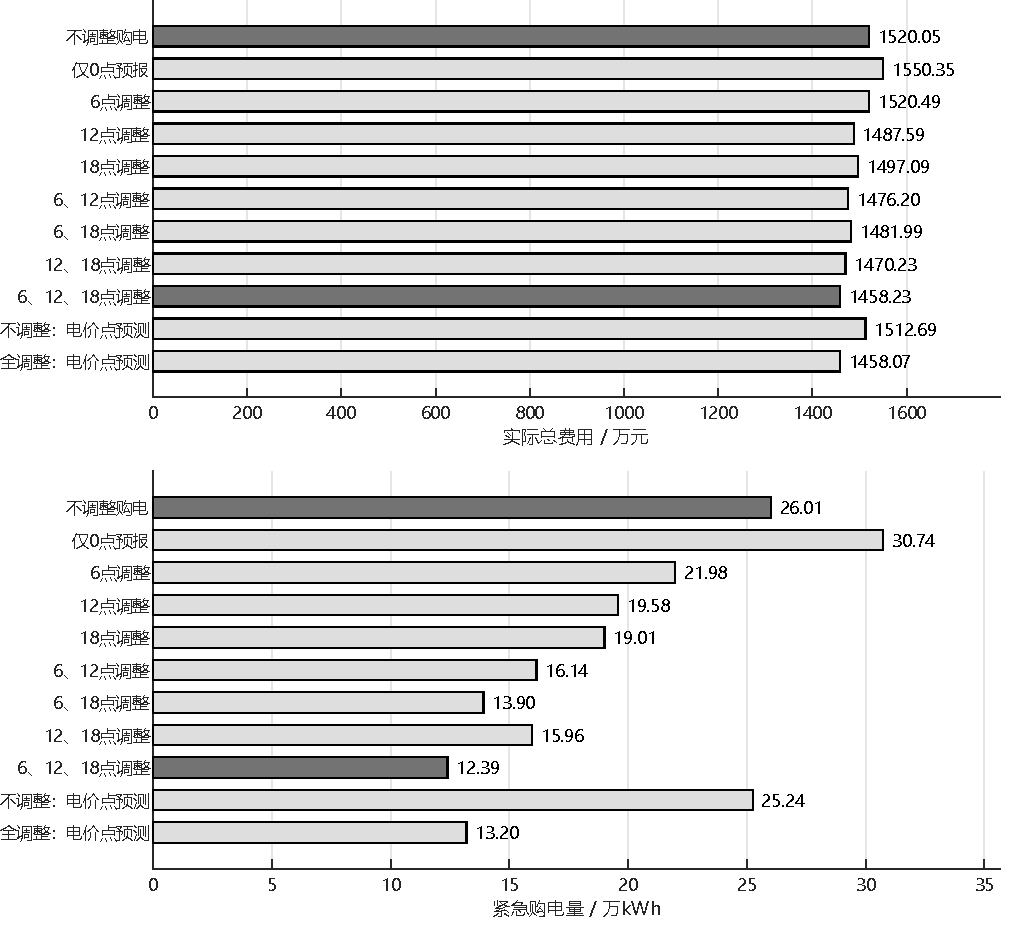
\includegraphics[width=\textwidth,height=.68\textheight,keepaspectratio]{figures/q4_compare.pdf}
\caption{波动电价下各策略的实际费用与紧急购电量。灰色深浅用于突出两组主方案。}\label{fig:q4compare}
\end{figure}
\begin{figure}[htbp]\centering
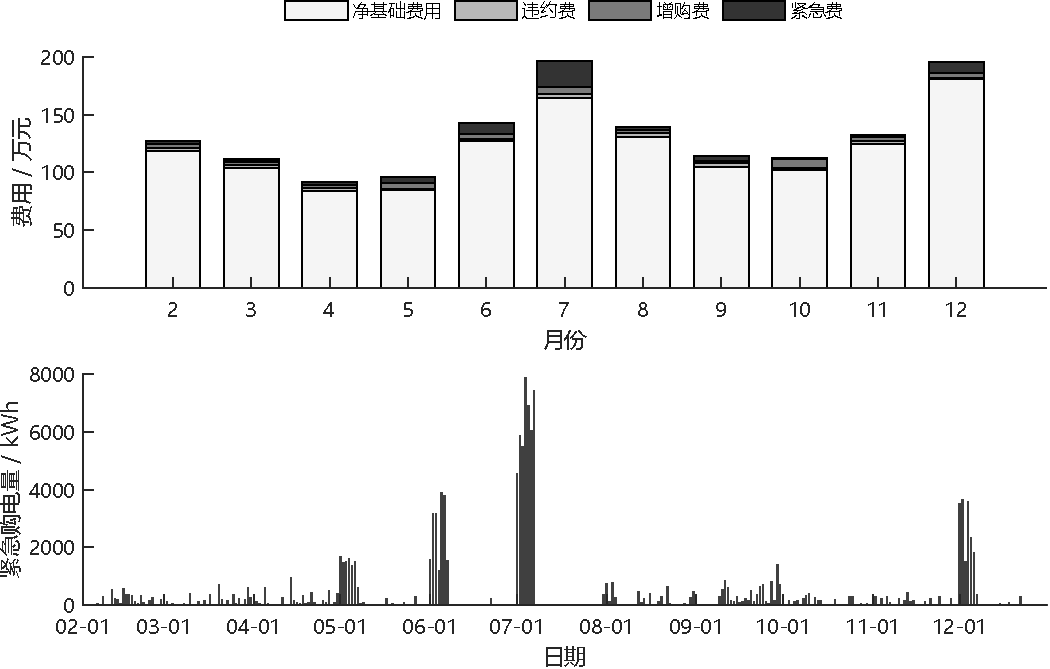
\includegraphics[width=\textwidth,height=.48\textheight,keepaspectratio]{figures/q4_year.pdf}
\caption{全部日内预报方案的月度费用构成与每日紧急购电分布。}\label{fig:q4year}
\end{figure}

\subsubsection{指定日期的购电与储能安排}
表\ref{tab:q4two_selected}和表\ref{tab:q4three_selected}分别汇总不调整与允许调整两组主方案的指定日结果。无调整策略的最终有效量等于原计划量；允许调整时，原计划金额与最终总费用不能相加。
\begin{table}[htbp]\centering\scriptsize
\caption{波动电价下不调整购电的指定日汇总（电量单位：kWh）}\label{tab:q4two_selected}
\resizebox{\textwidth}{!}{\begin{tabular}{lrrrrrr}
\toprule
日期 & 原计划量 & 最终有效量 & 紧急量 & 费用/元 & 日初电量 & 日末电量 \\
\midrule
03-20 & 66684.3799 & 66684.3799 & 302.4352 & 44055.5496 & 4744.4468 & 2800.5927 \\
06-21 & 38458.8333 & 38458.8333 & 0.0000 & 20398.6189 & 5060.0210 & 5768.8818 \\
09-23 & 69350.3802 & 69350.3802 & 764.5744 & 49312.1315 & 3425.1729 & 3827.7292 \\
12-21 & 98821.0250 & 98821.0250 & 0.0000 & 75309.9166 & 7993.7128 & 7835.3591 \\
\bottomrule
\end{tabular}
}
\end{table}
\begin{table}[htbp]\centering\scriptsize
\caption{波动电价下允许调整购电的指定日汇总（电量单位：kWh）}\label{tab:q4three_selected}
\resizebox{\textwidth}{!}{\begin{tabular}{lrrrrrr}
\toprule
日期 & 原计划量 & 最终有效量 & 紧急量 & 费用/元 & 日初电量 & 日末电量 \\
\midrule
03-20 & 67769.7059 & 62859.7913 & 697.6209 & 45519.6014 & 6895.4626 & 4175.8209 \\
06-21 & 36542.1857 & 36472.1998 & 0.0000 & 19294.6432 & 4405.3496 & 5318.7282 \\
09-23 & 71237.4855 & 66072.3836 & 640.6142 & 48801.3707 & 1380.6284 & 1799.0836 \\
12-21 & 97093.9992 & 96922.4053 & 0.0000 & 73756.5780 & 9079.9933 & 8658.8877 \\
\bottomrule
\end{tabular}
}
\end{table}
\begin{table}[htbp]\centering\small
\caption{不调整购电策略的六个指定时段购电量（kWh）}
\begin{tabular}{llrrrr}
\toprule
区间 & 电量类型 & 03-20 & 06-21 & 09-23 & 12-21 \\
\midrule
10:00--10:10 & 原计划 & 0.0000 & 0.0000 & 0.0000 & 0.0000 \\
12:00--12:10 & 原计划 & 670.4659 & 0.0000 & 601.0100 & 834.2664 \\
14:00--14:10 & 原计划 & 0.0000 & 0.0000 & 0.0000 & 0.0000 \\
16:00--16:10 & 原计划 & 419.6789 & 0.0000 & 634.6116 & 827.2097 \\
18:00--18:10 & 原计划 & 0.0000 & 514.7348 & 0.0000 & 743.1626 \\
20:00--20:10 & 原计划 & 720.7420 & 0.0000 & 292.7097 & 0.0000 \\
\bottomrule
\end{tabular}

\end{table}
\begin{table}[htbp]\centering\small
\caption{允许调整策略的六个指定时段原计划与最终有效量（kWh）}
\begin{tabular}{llrrrr}
\toprule
区间 & 电量类型 & 03-20 & 06-21 & 09-23 & 12-21 \\
\midrule
10:00--10:10 & 原计划 & 0.0000 & 0.0000 & 0.0000 & 0.0000 \\
10:00--10:10 & 最终有效 & 0.0000 & 0.0000 & 0.0000 & 0.0000 \\
12:00--12:10 & 原计划 & 571.9629 & 0.0000 & 624.5321 & 965.0345 \\
12:00--12:10 & 最终有效 & 501.2602 & 0.0000 & 289.1501 & 965.0345 \\
14:00--14:10 & 原计划 & 0.0000 & 0.0000 & 0.0000 & 0.0000 \\
14:00--14:10 & 最终有效 & 0.0000 & 0.0000 & 0.0000 & 0.0000 \\
16:00--16:10 & 原计划 & 692.1818 & 105.8485 & 495.8757 & 852.0926 \\
16:00--16:10 & 最终有效 & 512.0988 & 105.8485 & 495.8757 & 852.0926 \\
18:00--18:10 & 原计划 & 0.0000 & 480.2305 & 0.0000 & 696.6572 \\
18:00--18:10 & 最终有效 & 0.0000 & 460.2984 & 0.0000 & 679.2063 \\
20:00--20:10 & 原计划 & 0.0000 & 0.0000 & 746.8318 & 0.0000 \\
20:00--20:10 & 最终有效 & 38.0099 & 0.0000 & 731.6420 & 0.0000 \\
\bottomrule
\end{tabular}

\end{table}
各四小时时段的充放电量及连续紧急购电区间见附录\ref{app:q4selected}。所有表格来自对应全年连续回测，日初储电量取前一日真实执行的日末值。

\begin{figure}[htbp]\centering
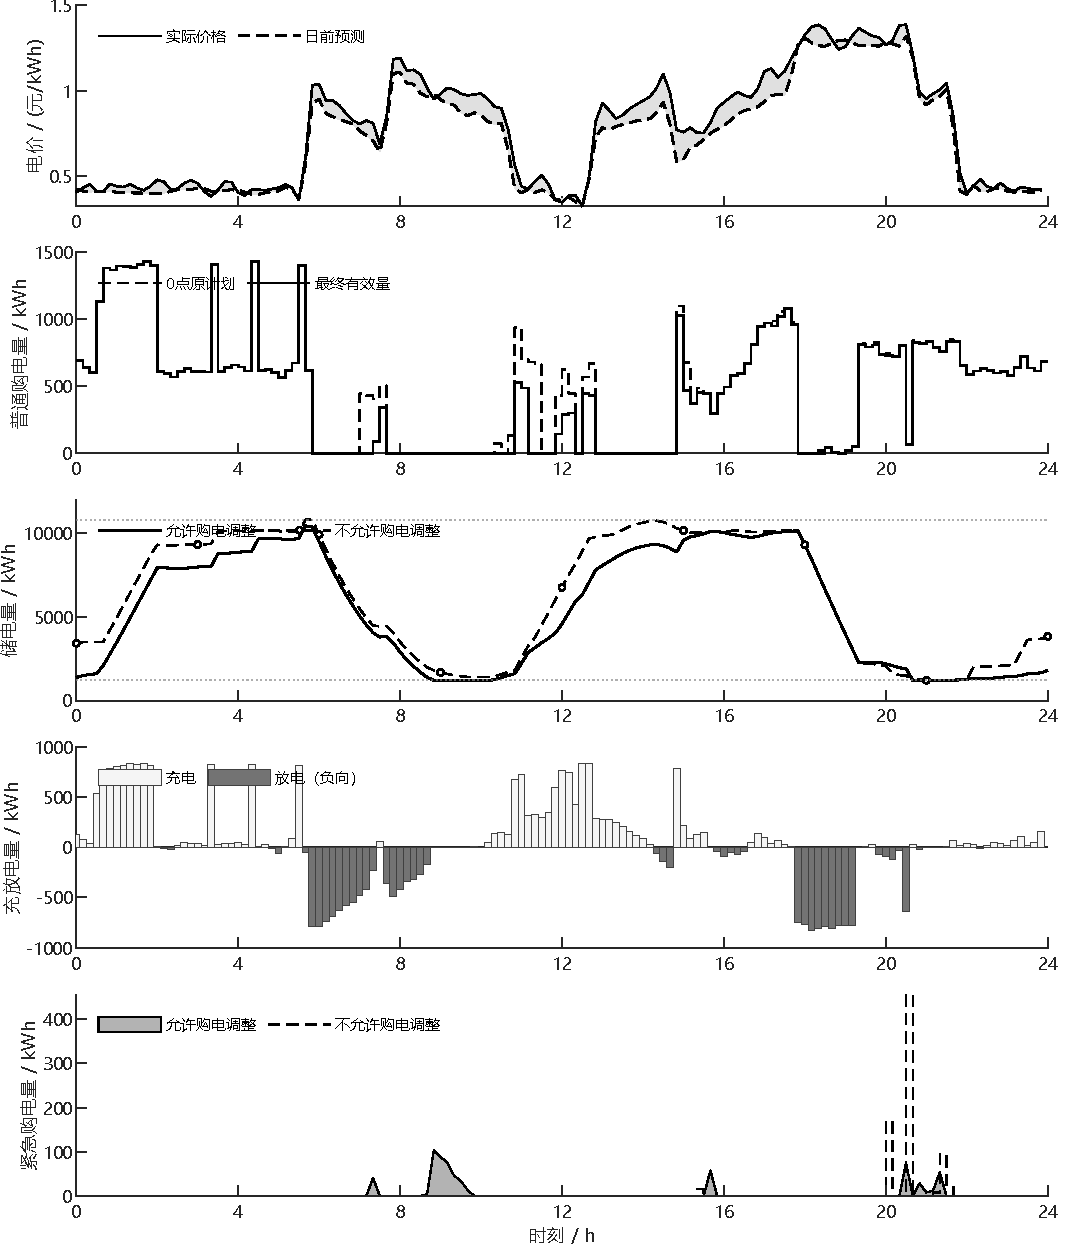
\includegraphics[width=\textwidth,height=.84\textheight,keepaspectratio]{figures/q4_day_20250923.pdf}
\caption{9月23日的电价预测、购电修订与储能响应。价格图的浅灰区域表示实际价格与日前预测之间的差异。两组策略分别沿用各自连续回测的日初状态。}\label{fig:q4response}
\end{figure}
